\documentclass[english]{scrartcl}
\usepackage[T1]{fontenc}
\usepackage[utf8]{inputenc}
\usepackage[scaled=.8]{beramono}
\usepackage{geometry}
\geometry{verbose,tmargin=3cm,bmargin=3cm,lmargin=3cm,rmargin=3cm}
\usepackage{microtype}
\usepackage[parfill]{parskip}
\usepackage{amsmath}
\usepackage{graphicx}
\usepackage{hyperref}
\usepackage{nameref}
\usepackage{float}
\usepackage{listings}
\usepackage{color}
\usepackage{fancyhdr}
\usepackage{blindtext}

\usepackage{subcaption}

\pagestyle{fancy}
\fancyhf{}
\rhead{Group 2}
\lhead{DM: Subspace Clustering}
\cfoot{\thepage}

\newcommand*{\fullref}[1]{\hyperref[{#1}]{\autoref*{#1}~\nameref*{#1}}}

\definecolor{darkgray}{rgb}{0.66, 0.66, 0.66}
\definecolor{asparagus}{rgb}{0.53, 0.66, 0.42}

\lstdefinestyle{s}{
  commentstyle=\color{darkgray},
  keywordstyle=\bfseries,
  morekeywords={},
  stringstyle=\color{asparagus},
  basicstyle=\ttfamily\footnotesize,
  breakatwhitespace=false,
  keepspaces=true,
  numbersep=5pt,
  showspaces=false,
  showstringspaces=false,
}

\lstset{style=s}

\begin{document}

\title{Data Mining\\Programming Assignment 1: Subspace Clustering}

\author{Sonja Biedermann \and Thilo Hannes Fryen \and Chan Dat Dennis Huyen \and David Turner}

\maketitle
\tableofcontents

\section{ORCLUS}

We decided to implement the ORCLUS algorithm. ORCLUS is a spin on $k$-means
which utilizes eigensystems to adapt the distance measure to non axis parallel
correlation clusters.

We picked this algorithm because the paper is easy to read and contains good
pseudocode which is of utmost importance when trying to actually implement
the described algorithm.

Furthermore, since $k$-means was the first clustering algorithm we studied, it will forever
have a special Gaussian-shaped spot in our heart---which makes ORCLUS, as a
spiritual successor, a natural choice.

\subsection{Description and Pseudocode}

The algorithm proceeds in rounds in which the dimensionality of the clusters
and the number of clusters is gradually reduced. The rate at which this happens should
not be too quickly, to which end the authors propose two parameters $\alpha$ and $\beta$
and a relation between these two, by which one can be calculated from the other. They
suggest an $\alpha$ of 0.5, which we've also adopted.

In each round, the algorithm undertakes an assignment step which is the same as
in $k$-means. Every point is assigned to the closest centroid. However, as a
next step, the eigenvectors associated with the smallest spread are computed on
a per cluster basis---the rationale behind this is that those vectors define a
subspace in which the points cluster well, i.e. have a low contribution to the
overall cluster energy. The cardinality of this vector set dictates the dimensionality
of the subspace to which the points are projected.

To reduce the amounts of clusters---the algorithm starts with more seeds than
requested by the user, we've chosen to start with 5 times as many as the
authors offer no suggestions---a merging step is performed next. Although quite
lengthy, this operation is pretty simple. The objective is to find pairs of
clusters which can be merged such that the overall cluster energy stays low.
For this, all pairs of clusters are examined, their centroid and energy
computed and then the cluster-pairs with the lowest energy are picked to be merged, being
careful to update all relevant data structures after each merge.

These three steps are repeated until the desired dimensionality and number of
clusters are reached. After a final assignment step the clustering is returned.

%% TODO: pseudocode

\subsection{Implementation}

We chose to implement the algorithm in Python 3. The implementation is rather straight
forward and only depends on NumPy and some functionality from Python's standard
library.

Notably we use \texttt{numpy.linalg.eigh} to decompose the cluster matrices
into eigenvalues and eigenvectors. We know PCA could also be used but online
literature\footnote{\url{https://stackoverflow.com/questions/50358310/how-does-numpy-linalg-eigh-vs-numpy-linalg-svd}}
suggests that the LAPACK routines utilized in NumPy's implementation of
\texttt{eigh} perform a tiny sliver better than SVD, which we expect to be used
in \texttt{sklearn.decomposition.PCA}.  However, this probably would make no
practical difference whatsoever.

The initial seeds are distributed using the kmeans\texttt{++} initialization strategy,
although we have also implemented a completely random initalization strategy.
If the initial seed count is chosen to be high enough, this strategy actually
seems to be beneficial, as it returns good partitions and is also faster.

\section{Evaluation}

We will be comparing ourselves to the ELKI implementation on 4 synthetic datasets
using the NMI as scoring method. The datasets were generated using ELKI's data generator.
We used flat Gaussian distributions as correlation clusters and added noise points
to disturb the algorithm.

\subsection{Simple dataset}

As a simple first dataset we feed a 2-dimensional data set containing 3 clusters that are very clearly
separated, one of which is a bit fatter than the stereotypical correlation cluster, but which is
axis-parallel. Figure~\ref{fig:test} shows the results obtained by our implementation (Figure~\ref{fig:test-ours})
and the result obtained by the implementation contained in ELKI. They are identical---notably misclassifying one
single point which would belong to the fat axis-parallel cluster.

\begin{figure}[tb]
    \centering
    \begin{subfigure}[t]{0.5\textwidth}
        \centering
        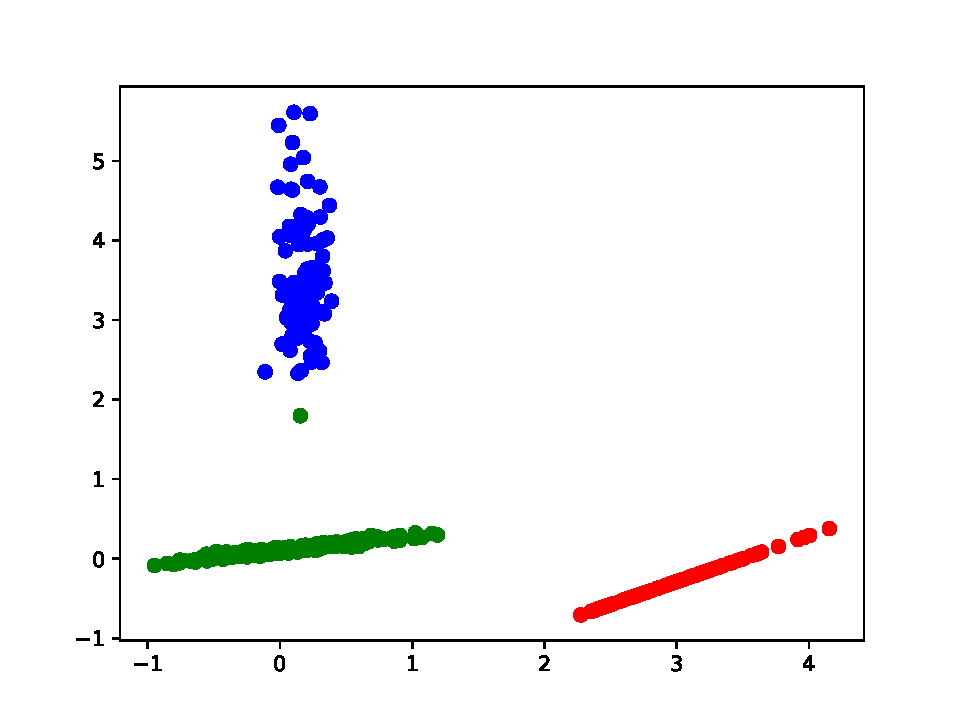
\includegraphics[width=\textwidth]{img/test_ours}
        \caption{Our implementation}
        \label{fig:test-ours}
    \end{subfigure}%
    \begin{subfigure}[t]{0.5\textwidth}
        \centering
        
\includegraphics[width=2\textwidth]{img/test_elki}
        \caption{ELKI's implementation}
    \end{subfigure}

    \caption{Bla}
    \label{fig:test}
\end{figure}

\subsection{Simple dataset with added noise}

% coming soon

\subsection{Clusters that are noise in some subspaces}

% coming soon

\subsection{Clusters with different rotations in some subspaces}

% coming soon

\subsection{Summary}

% also coming soon

\end{document}
